\documentclass{article}
\usepackage[utf8]{inputenc}
\usepackage{graphicx}
\graphicspath{ {images/} }
\usepackage{multicol}
\setlength{\columnsep}{2cm}

\documentclass[12pt]{article}
\usepackage[cp1251]{inputenc}
\usepackage[russian]{babel}
\begin{document}

\begin{titlepage}
	\centering
	{\scshape\LARGE Московский физико-технический институт \par}
	\vspace{3cm}
	{\scshape\Large Лабораторная работа \par}
	\vspace{1cm}
	{\huge\bfseries Определение теплопроводности воздуха при атмосферном давлении \par}
	\vspace{1cm}
	\vfill
\begin{flushright}
	{\large выполнила студентка 653 группы ФФКЭ}\par
	\vspace{0.3cm}
	{\LARGE Карпова Татьяна}
\end{flushright}
	

	\vfill

% Bottom of the page
	Долгопрудный, 2017 г.
\end{titlepage}

\section{Цель работы}
Определение коэффициента теплопроводности воздуха при атмосферном давлении и разных температурах по теплоотдаче нагреваемой током нити в цилиндрическом сосуде

\section{В работе используются}
\begin{itemize}
    \item прибор для определения теплопроводности газов
    \item форвакуумный насос
    \item термостат
    \item магазин сопротивлений
    \item цифровой вольтметр В7-38
    \item эталонное сопротивление 10 Ом
    \item источник питания
    
\end{itemize}

\section{Теоретические положения}

{\it Теплопроводность} --- процесс, приводящий к выравниванию температуры в сосуде, где температура залючённого газа зависит от координат. Теплопроводность связана с тепловым движением молекул и не сопровождается макроскопическими перемещениями газа. \par
{\it Коэффициент теплопроводности} --- основная характеристика теплопроводности --- это коэффициент пропорциональности между плотностью потока тепла $q$ и градиентом температуры $dT/dr$ в направлении этого потока:
\begin{center}
$q = -\kappa \frac{dT}{dr}$
\end{center} \par

В цилиндрически симметричной установке, в которой тепловой поток направлен к стенкам цилиндра от нити, полный поток тепла $Q = qS$ через каждую цилиндрическую поверхность радиуса $r$ должен в стационарном состоянии быть неизменен в пространстве и во времени. Тогда
\begin{center}
$Q = -2\pi r L \kappa \frac{dT}{dr} = const$,
\end{center}
откуда получаем
\begin{center}
$T_1 - T_2 = \frac{Q}{2\pi L \kappa} ln\frac{R}{r}$
\end{center}\par
 В нашем эксперименте необходимо найти
 \begin{center}
 \begin{equation}
 \kappa = \frac{Q}{T_1-T_2}\frac{1}{2\pi L}ln \frac{r2}{r1}
 \end{equation}
 \end{center}
 
 \section{Экспериментальная установка}
 Схема лабораторной установке представлена на рисунке 1. Тонкая молибденовая проволока натянута по оси вертикально стоящей медной трубки. Через штуцер трубка заполняется исследуемым газом. Нить нагревается электрическим током, ее температура $T_1$ определяется по изменению электрического сопротивления. Трубка находится в кожухе, через который пропускается вода из термостата. Температура воды $T_2$ измеряется термометром, помещенным в термостат. Количество теплоты,
протекающей через газ, равно (если пренебречь утечками тепла через торцы) количеству теплоты, выделяемому током в нити, и может быть найдено по закону Джоуля—Ленца. При этом ток в нити определяется по напряжению на включенном последовательно с ней эталонном сопротивлении 10 Ом. Таким образом, все величины, входящие в правую часть формулы (1), поддаются непосредственному измерению. \par
Электрическая часть схемы состоит из источника питания и под-
ключенных к нему последовательно соединенных нити, эталонного
сопротивления 10 Ом и магазина сопротивлений $R_M$, служащего для
точной установки тока через нить. Цифровой вольтметр может под-
ключаться как к нити, так и к эталонному сопротивлению, измеряя
таким образом напряжение на нити и ток через нее.

\begin{figure}[h]
    \centering
    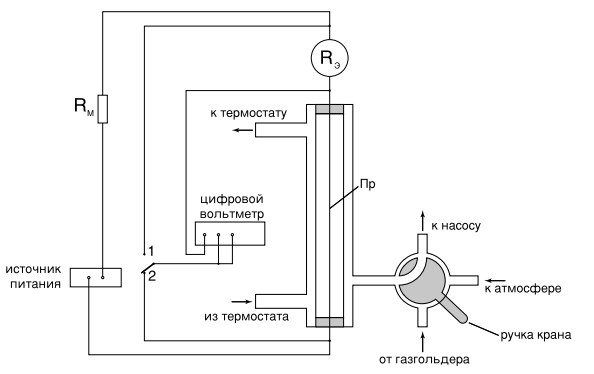
\includegraphics[width=7.5 cm]{setup.PNG}
    \caption{Схема установки для определения теплопроводности газов}
    \label{fig:vac}
\end{figure}

 \section{Ход работы}
\begin{enumerate}
     \item Определим параметры экспериментальной установки:
     \begin{multicols}{2}
     $L$ = 347 мм\\
     $2r_1$ = 0,055 мм\\
     $2r_2$ = 10 мм\\
     $R_0$ = 10 Ом\\
     класс точности 0,01
     \end{multicols}
     
     \item Проведём измерения зависимости падения напряжений от температуры молибденовой нити. Для этого будем устанавливать с помощью магазина напряжений различные напряжения в цепи в интервале от 0,1 до 1,5 В и затем переносить штекер от вольтметра на прибор для измерения теплопроводности. Зависимость снимем для различных температур в интервале от 25 до 60 градусов. Результаты измерений занесём в таблицу 1. \par
     Сопротивление нити рассчитывается по формуле $R_H = R_0 \frac{U_H}{U_0}$. Выделяемая мощность рассчитывается по формуле $Q = \frac{U_H U_0}{R_0}$. Эти значения также занесём в таблицу 1.
     
     \begin{table}[t]
    \centering
    \caption{Значения напряжения на установке, сопротивления нити и выделяемой на ней мощности от температуры нити}
    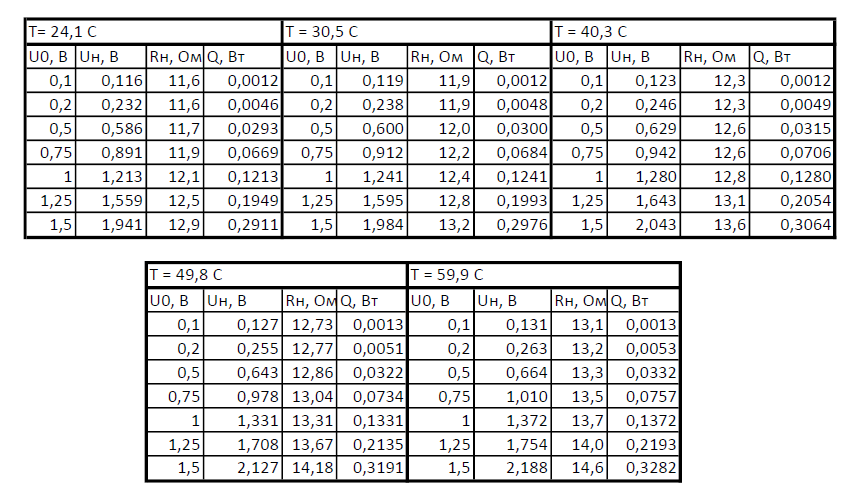
\includegraphics[width=\textwidth]{table1.PNG}
    \label{fig:vac}
    \end{table}
     
     \item Для каждой серии измерений построим график зависимости выделяемой мощности от сопротивления нити. По графику определим наклон $dQ/dR$ и сопротивление нити при температуре термостата (при Q = 0). \par 
     \begin{center}
     Т = 24,1 С:\hspace{1cm}$dQ/dR = 0.2153$, $R_0 = 11.57$ Ом\\
     Т = 30,5 С:\hspace{1cm}$dQ/dR = 0.22$, $R_0 = 11.87$ Ом\\
     Т = 40,3 С:\hspace{1cm}$dQ/dR = 0.2314$, $R_0 = 12.29$ Ом\\
     Т = 49,8 С:\hspace{1cm}$dQ/dR = 0.2218$, $R_0 = 12.72$ Ом\\
     Т = 59,9 С:\hspace{1cm}$dQ/dR = 0.2296$, $R_0 = 13.13$ Ом\\ 
     \end{center}
     
         \begin{figure}[H]
    \centering
    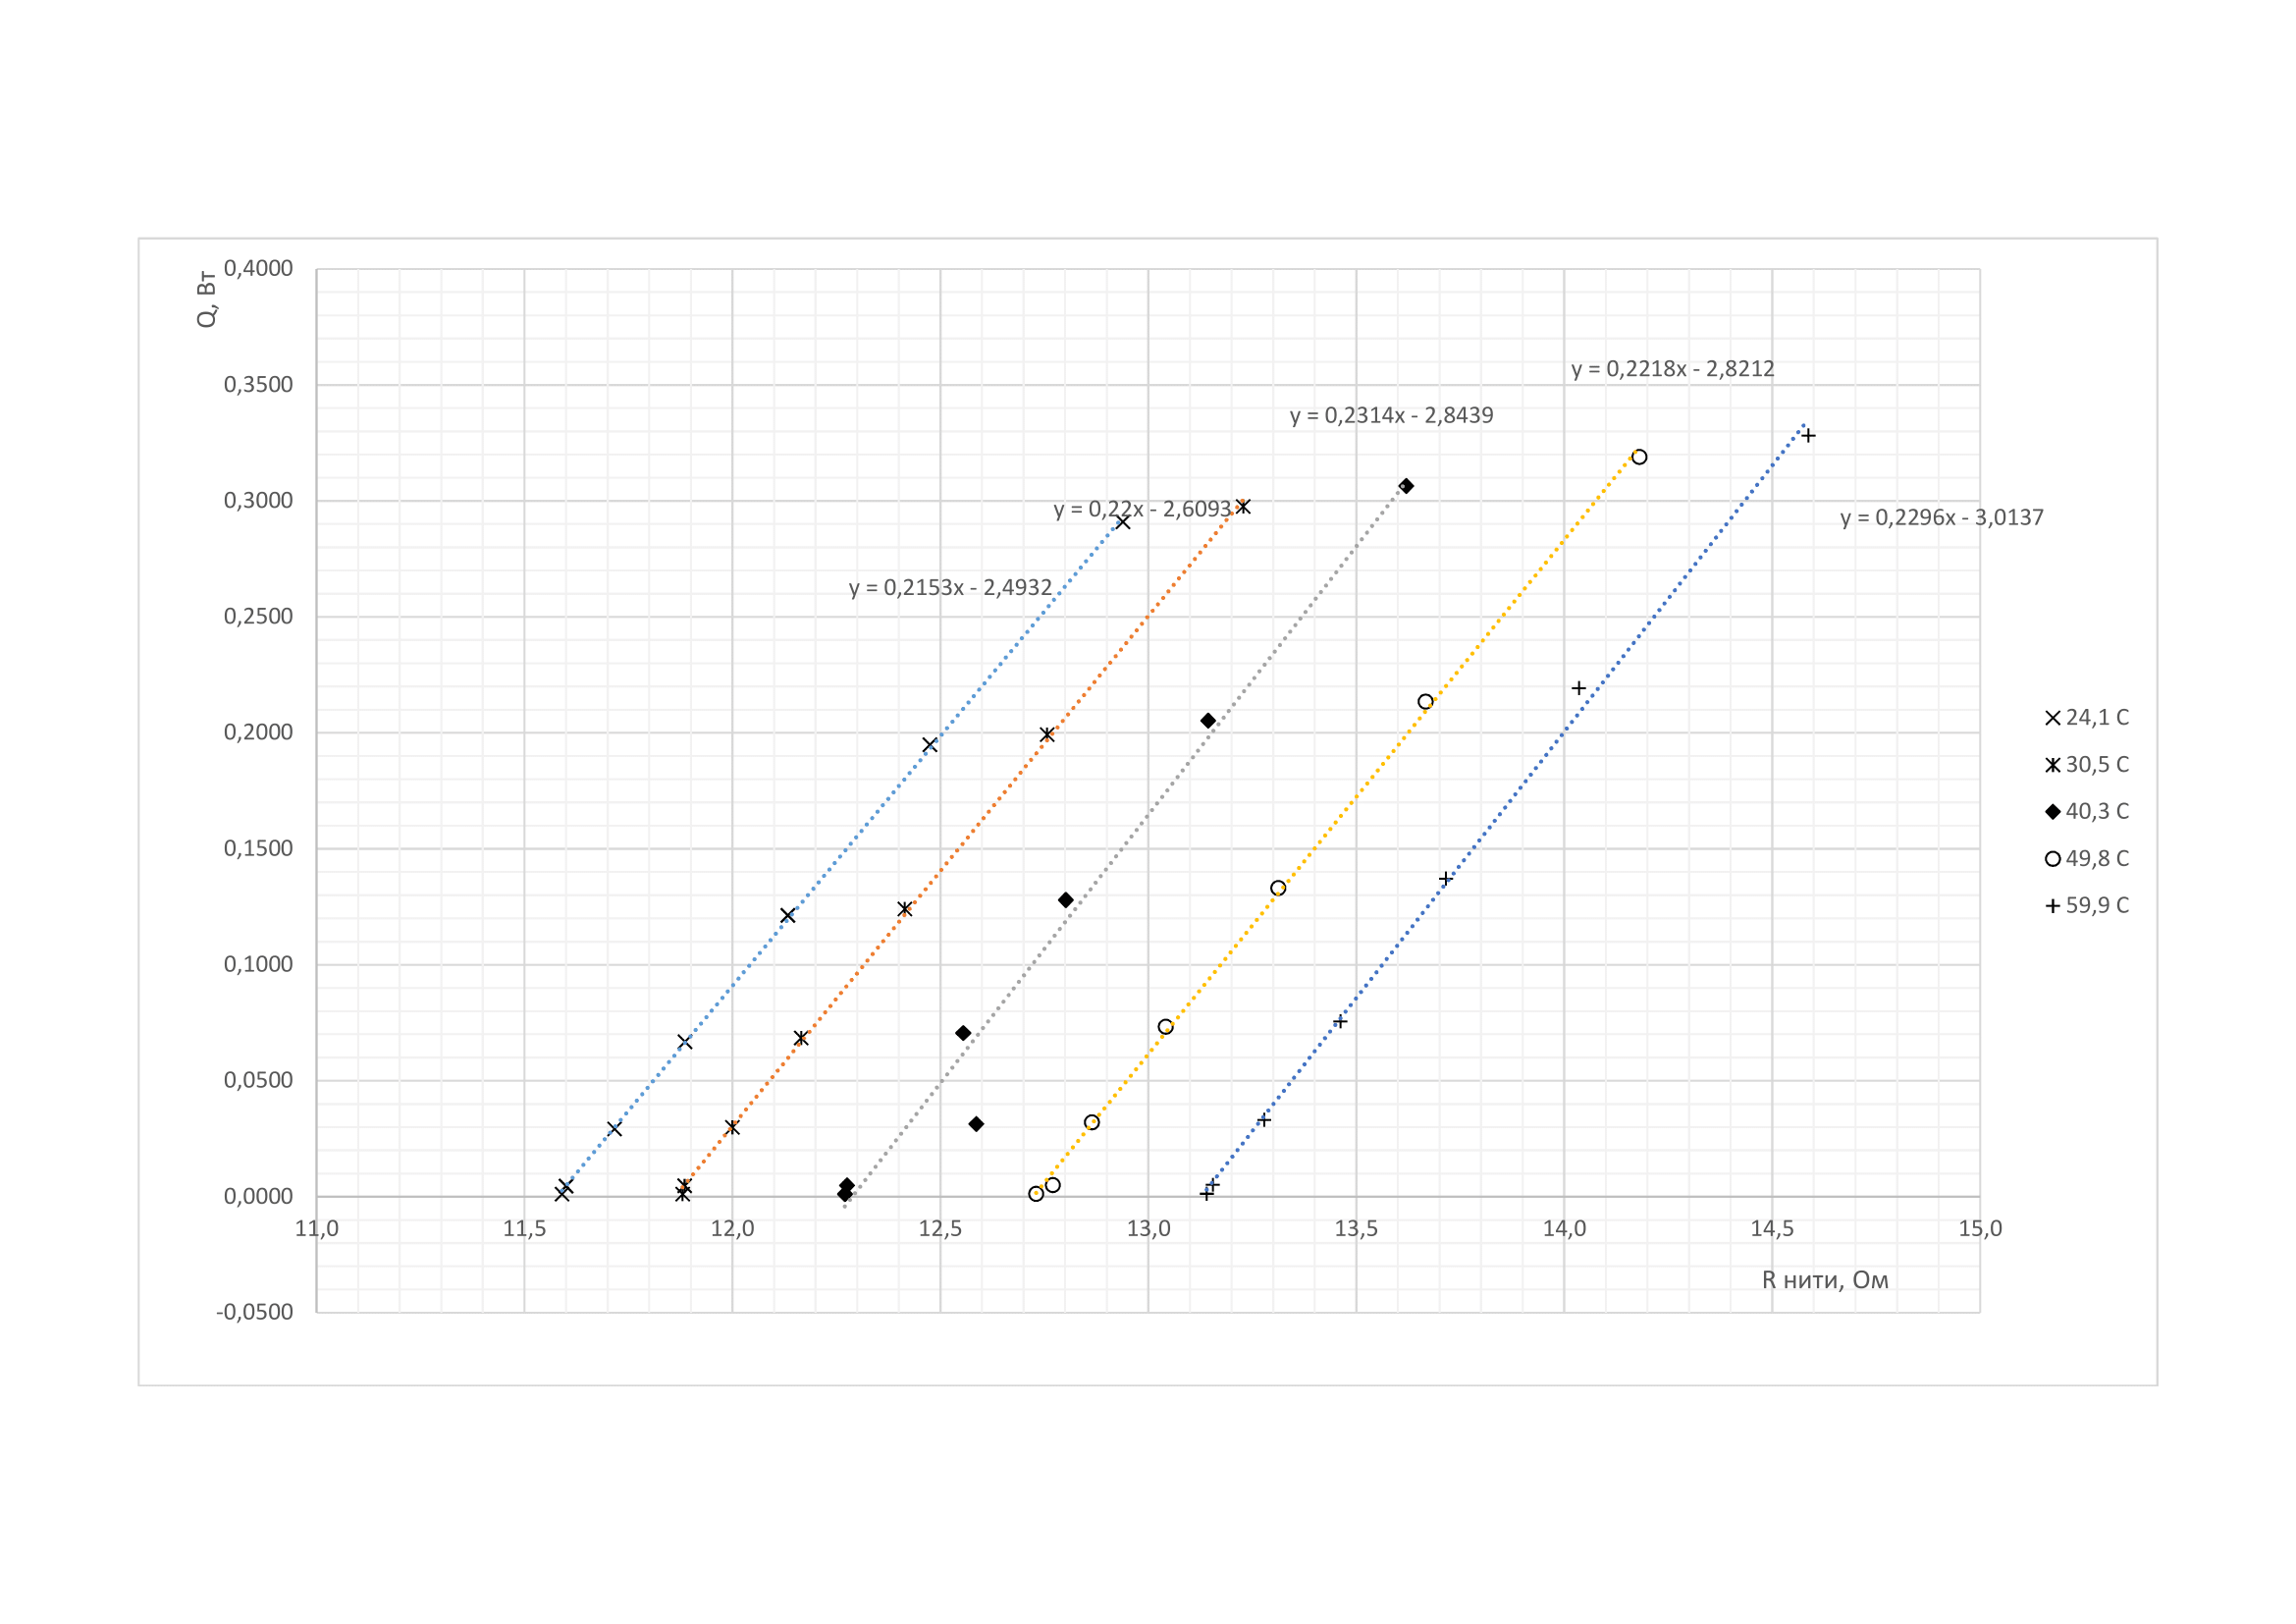
\includegraphics[width=20cm, angle=90]{graph-1.png}
    \caption{Зависимость выделяемой мощности от сопротивления нити}
    \label{fig:vac}
    \end{figure}
     
     \item Проанализируем график. Мы видим, что с повышением температуры угол наклона прямой Q(R) увеличивается, но на температуре 49,8 С зависимость нарушается: коэффициент угла наклона уменьшается. Это явление можно объяснить проявлением конвекции при достижении воздухом в установке достаточно высокой температуры: часть тепловой энергии переносится от нити к стенке именно этим путём. Поэтому нет ничего удивительного, что результаты при высоких температурах отличаются от ожидаемых, график должен "опутиться". 
     
     \item Оценим погрешность измерений. Погрешность измерений выделяемой мощности оценим по формуле
     \begin{center}
     $\sigma Q = Q\sqrt{(\frac{\sigma U_H}{U_H})^2+(\frac{\sigma U_0}{U_0})^2+(\frac{\sigma R_0}{R_0})^2}$
     \end{center} \par
     
     Погрешность измерений сопротивления нити оценим по формуле 
     \begin{center}
     $\sigma R = R\sqrt{(\frac{\sigma U_H}{U_H})^2+(\frac{\sigma U_0}{U_0})^2+(\frac{\sigma R_0}{R_0})^2}$
     \end{center} \par
     
     Также оценим влияние потерь тепла через концы проволоки. Рассчитаем количество тепла, отводимое с двух концов молибденовой проволоки длиной 1 см каждый, зная разность комнатной температуры и температуры воздуха в установке. \par
     Формула для мощности тепловых потерь в результате теплопроводности:
     \begin{center}
     $Q = - \kappa \frac{S \triangle T}{L}$,
     \end{center}
     где $\kappa$ - теплопроводность металла, $S = \pi r^2$ - площадь поперечного сечения образца, $L$ - его длина, $\triangle T$ - разность температур.
     
     Результаты вычисления погрешностей занесём в таблицу 2. 
     

    
    Видим, что при большом перепаде температур при небольших напряжениях потери на теплопроводность металла играют огромную роль и составляют до половины значения, регистрируемого на вольтметре. Также при небольших напряжениях наблюдаем большую погрешность измерений (13\%), при повышении напряжения погрешность уменьшается до порядка 1\%
    
    \item По значениям $R_0$ из п.3 построим график зависимости сопротивления молибденовой нити от температуры. 
    
    \begin{table}[H]
    \centering
    \caption{Погрешности определения мощности потерь, сопротивления проволоки и учёт теплопроводности проволоки}
    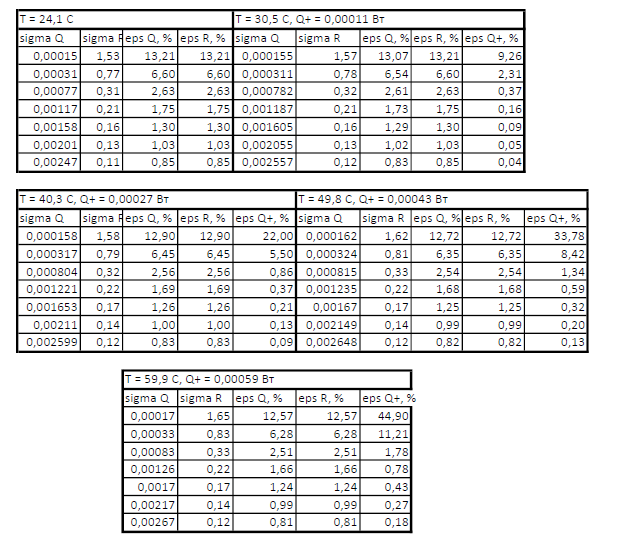
\includegraphics[width=14cm]{table2.PNG}
    \label{fig:vac}
    \end{table}
     
    \begin{figure}[h]
    \centering
    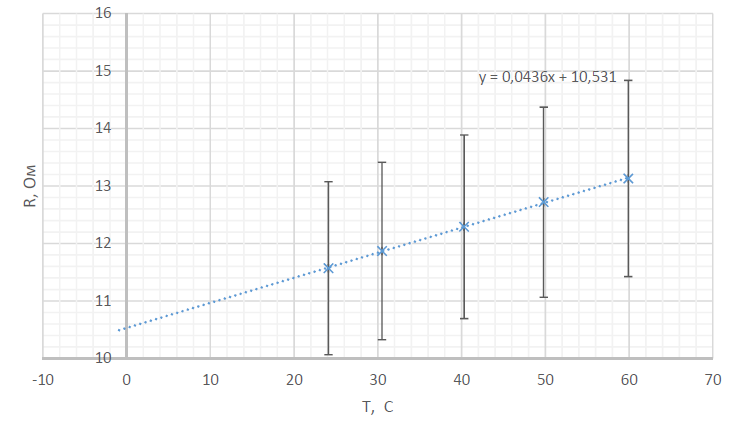
\includegraphics[width=7.5 cm]{graph2.PNG}
    \caption{График зависимости сопротивления нити от температуры}
    \label{fig:vac}
    \end{figure}
    
    Погрешность измерения сопротивления при напряжении 0,1 В составляет 13\%, примерно такую же погрешность будут иметь и точки на графике и, следовательно, полученный коэффициент ($dR/dT$).
    
    \item По графику на рис. 3 определим значение температурного коэффициента сопротивления материала нити - молибдена:
    \begin{center}
    $\alpha = \frac{1}{R_0C}\frac{dR}{dT} = 0.00414$  $K^-^1 $\\
    \end{center}
    С учётом погрешности величин:
    \begin{center}
    $\alpha = 0.00414 \pm 0.00076$ $K^-^1 $ \\
    \end{center}
    
    Табличное значение температурного коэффициента молибдена составляет 0.004579 $K^-^1$. Полученный нами результат совпадает с табличным в пределах допустимой погрешности.
    
    \item Для каждого значения температуры определим значение теплопроводности газа по формуле, учтём погрешности из предыдущих пунктов
    \begin{center}
    $\kappa = \frac{dQ}{dR} \frac{dR}{dT} \frac{1}{2 \pi L} ln\frac{r_2}{r_1}$
    \end{center}
    
    \begin{center}
     Т = 24,1 С:\hspace{0.5cm}$\kappa = 0.02186 \pm 0.0040$ Вт/м*С\hspace{0.5cm}$\kappa_T = 0.00262$ Вт/м*С\\
     Т = 30,5 С:\hspace{0.5cm}$\kappa = 0.02290 \pm 0.0042$ Вт/м*С\hspace{0.5cm}$\kappa_T = 0.00267$ Вт/м*С\\
     Т = 40,3 С:\hspace{0.5cm}$\kappa = 0.02409 \pm 0.0044$ Вт/м*С\hspace{0.5cm}$\kappa_T = 0.00276$ Вт/м*С\\
     Т = 49,8 С:\hspace{0.5cm}$\kappa = 0.02309 \pm 0.0043$ Вт/м*С\hspace{0.5cm}$\kappa_T = 0.00283$ Вт/м*С\\
     Т = 59,9 С:\hspace{0.5cm}$\kappa = 0.02390 \pm 0.0044$ Вт/м*С\hspace{0.5cm}$\kappa_T = 0.00290$ Вт/м*С\\ 
     \end{center}
    
   \par  Видим, что значения сходятся с табличными по порядку величины, и, учитывая погрешность измерений, практически совпадают с ними. При больших температурах не прослеживается возрастание полученных экспериментально значений, так как не учтена роль конвекции (если учесть эти потери, значения окажутся ближе к реальным). \par
   
   Построим на одном графике теоретическую зависимость коэффициента теплопроводности от температуры и полученную экспериментально (рисунок 4). По графику можно оценить влияние конвекции на ход эксперимента. Также наблюдается систематическая ошибка - экспериментальные значения "занижены" примерно на 0,004 Вт/м*С.
   
    \begin{figure}[H]
    \centering
    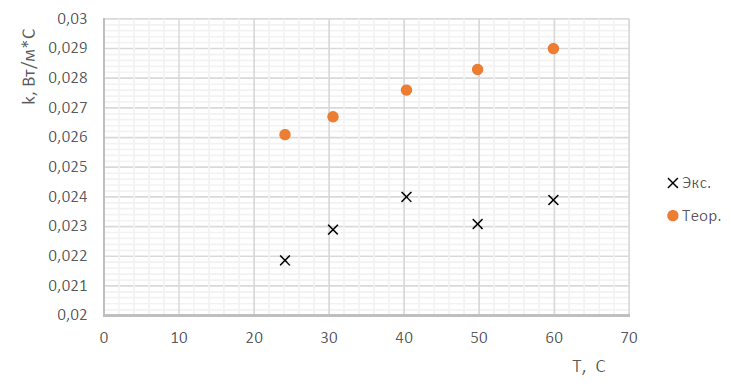
\includegraphics[width=\textwidth]{graph3.PNG}
    \caption{График зависимости коэффициента теплопроводности воздуха от температуры}
    \label{fig:vac}
    \end{figure}

    \item Предполагая, что зависимость коэффициента теплопроводности от температуры имеет вид $\kappa = AT^\beta $, определим показатель степени $\beta$. Для этого построим график зависимости $ln \kappa$ от $ln T$, тогда $ln\kappa = lnA + \beta lnT$
    
    \begin{figure}[H]
    \centering
    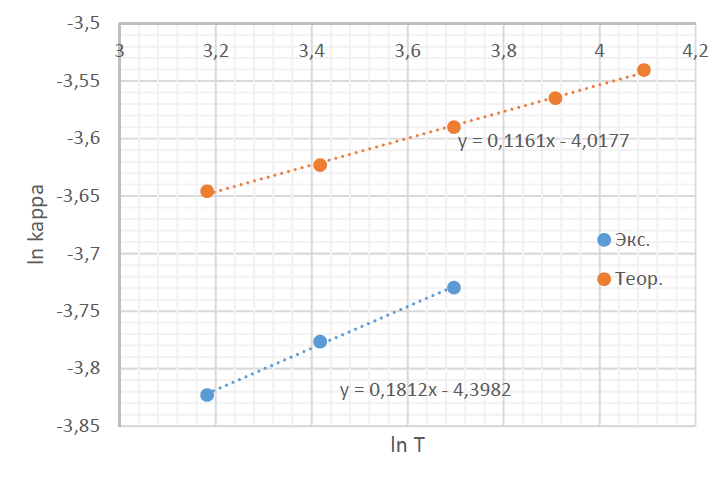
\includegraphics[width=\textwidth]{graph4.PNG}
    \caption{График зависимости натурального логарифма коэффициента теплопроводности воздуха от натурального логарифма температуры}
    \label{fig:vac}
    \end{figure}
    
    \item Получили, что коэффициент $\beta \approx 0,2$. Это неверно, так как в теории коэффициент теплопроводности газа прямо пропорционален корню его температуры. Интересно, что необходимое значение не получилось и при обработке теоретических значений. Расхождение, скорее всего, связано с неточностями при выполнении эксперимента и большой погрешностью измерений.
    \newpage
    
   \end{enumerate}  
    \section{Вывод}
    
    \begin{enumerate}

        \item В ходе работы была экспериментально определена теплопроводность воздуха при различных температурах, обнаружена линейная зависимость этих величин.
        \item Были оценены погрешности измерения зависимости сопротивления молибденовой нити и мощности, выделяющейся на ней. Обнаружено, что при напряжении порядка 0,1 В погрешность измерений является довольно большой (13\%), при дальнейшем увеличении напряжения ошибка составляет около 1\%. Основной вклад в величину погрешности вносит относительная погрешность измерения напряжения на эталонном сопротивлении: 0,1 В при классе точности прибора вольтметра 0,01 В
        \item Была оценена доля мощности потерь тепла через концы молибденовой проволоки. При повышении разности температур эта величина вносит существенный вклад в погрешность (до 50\% при разности температур порядка 40 С)
        \item Экспериментально с большой точностью было определено значение температурного коэффициента молибдена: значение, полученное нами, $\alpha = 0.00414 \pm 0.00076$ $K^-^1 $ при табличном значении  $\alpha = 0.004579 $ $K^-^1 $
        \item Было обнаружено влияние конвекции на значения коэффициента теплопроводности воздуха: значения "занижаются"; также обнаружена систематическая ошибка определения коэффициента теплопроводности: значения также оказываются меньше теоретических. Это может быть связано с различными потерями тепла в установке: конвекция, излучение, потери через концы проволоки.
        \item Была сделана попытка определить характер зависимости коэффициента теплопроводности газа от температуры. Полученное нами значение ($\kappa = AT^1^/^5 $) не сошлось с теоретическим ($\kappa = AT^1^/^2 $). Такое различие может быть связано с большими погрешностями при проведении эксперимента.
 \end{enumerate}

    
    
    


\end{document}
